\documentclass[11pt]{article}
\title{\textbf{Meccano octagons}}
\author{https://github.com/heptagons/meccano/octa}
\date{}

\usepackage{listings}
\usepackage{xcolor}
\definecolor{gray}{RGB}{245,245,245}

\lstset{
	backgroundcolor=\color{gray},
	frame=single,
	language=c,
	numbers=left,
	stepnumber=1
}

\usepackage[margin=0.75in]{geometry}

\usepackage{tikz}
\usetikzlibrary{math}

\usepackage{graphicx}

\begin{document}

\maketitle

\section{Meccano octagons}

\begin{figure}
\centering
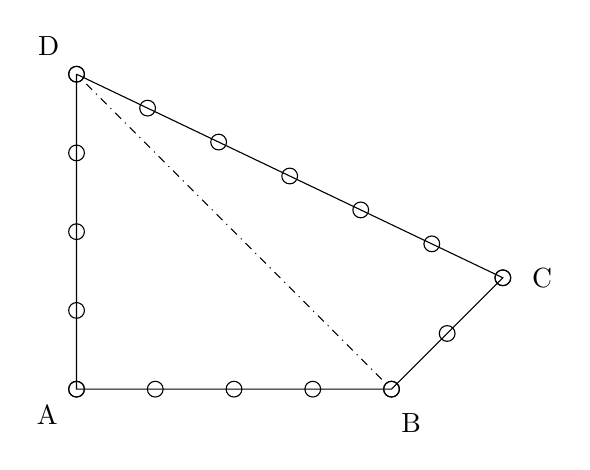
\begin{tikzpicture}

\foreach\x in {0,...,4} %AB
	\draw (\x,0) circle (0.1);

\tikzmath{
	\s = sqrt(2);
	for \x in {0,...,2}{ %BC
		{
			\draw (4 + \x*\s/2,\x*\s/2) circle (0.1);
		};
	};
	\x = 4 + \s;
	\cx = \x/6;
	\cy = (4 - \s)/6;
	for \c in {0,...,6}{ %CD
		{
			\draw (\x - \c*\cx, \s + \c*\cy) circle(0.1);
		};
	};
};

\foreach \d in {0,...,4} %DA
	\draw(0, 4-\d) circle (0.1);

\node (a) at (0,0) {};
\node (b) at (4,0) {};
\node (c) at ({4+sqrt(2)},{sqrt(2)}) {};
\node (d) at (0,4) {};
\node (e) at (3,0) {};

\draw[dash dot] (b) -- (d);

\path (a) ++(222:0.5) node{A};
\path (b) ++(-60:0.5) node{B};
\path (c) ++(0:0.5) node{C};
\path (d) ++(135:0.5) node{D};

\draw plot[] coordinates {
	(d) (a) (b) (c) (d)
};

\end{tikzpicture}
\caption{Meccano octagon plan. Isosceles right triangle $ABD$ has side equals to $4$ and hypothenuse $BD$ equals $4\sqrt{2}$. Next to this triangle we form another right triangle $BCD$ with sides $2$, $6$ and $4\sqrt{2}$. $ABC$ is the internal regular octagon angle since angle $ABC=45^{\circ}$ and $DBC=90^{\circ}$.
}
\label{fig:1}
\end{figure}

Figure \ref{fig:1} is the meccano octagon plan which joins two triangles to form an angle of $45^{\circ} + 90^{\circ}$.

\subsection{Finding octagons rods}

Next golang program find first cases:

\begin{lstlisting}
func octagons_2() {
  for i := 1; i < 60; i++ {
    for j := 1; j < i; j++ {
      test := i*i - j*j
      if test % 2 == 0 {
        f := math.Sqrt(float64(test / 2))
        k := int(f)
        if f == float64(k) {
           if gcd(k, gcd(j, i)) == 1 {
             fmt.Printf("CD=%2d BC=%2d AB=AD=%2d\n", i, j, k)
           }
        }
     }
   }
}
func gcd(a, b int) int {
  if b == 0 {
    return a
  } else {
    return gcd(b, a % b)
  }
}
\end{lstlisting}

The program iterates on $i$ and $j$ which corresponds to 
segments $\overline{CD}$ and $\overline{BC}$. Then the hipothenuse $\overline{DB}$ is checked
to be $\sqrt{2} \times \overline{AB}$ being $\overline{AB}$ and integer.

\subsection{Rods results}

Program's first results are:
\begin{lstlisting}
CD= 3 BC= 1 AB=AD= 2
CD= 9 BC= 7 AB=AD= 4
CD=11 BC= 7 AB=AD= 6
CD=17 BC= 1 AB=AD=12
CD=19 BC=17 AB=AD= 6
CD=27 BC=23 AB=AD=10
CD=33 BC=17 AB=AD=20
CD=33 BC=31 AB=AD= 8
CD=41 BC=23 AB=AD=24
CD=43 BC= 7 AB=AD=30
CD=51 BC=47 AB=AD=14
CD=51 BC=49 AB=AD=10
CD=57 BC= 7 AB=AD=40
CD=57 BC=41 AB=AD=28
CD=59 BC=41 AB=AD=30
\end{lstlisting}

\begin{figure}[htpb]
\centering
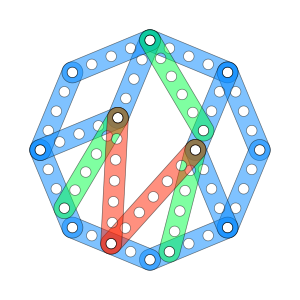
\includegraphics[]{figs/octagon-4}
\caption{Smallest octagon. From first result $CD=3, BC=1, AB=AD=2$,
we scale by 2 to get $CD=6, BC=2, AB=AD=4$ to have a buildable octagon.}
\label{fig:2}
\end{figure}

\subsection{Octagon of side 4}

At figure \ref{fig:2} we have the smallest octagon of length side $4$.
For this octagon we take the first result scaled by a factor of $2$ in order we can have a right triange large enough to be fixed by a $3-4-5$ triangle (hypothenuse in color green).

\begin{figure}
\centering
\begin{tikzpicture}[scale=0.5]
\tikzmath{
	\a = 5;\b = \a*sqrt(2)/2;
	\oa = 1;\ab = 6;\ad = 4;
	{\node (o) at (0,0) {};};
	{\node (a) at (\oa,0) {};};
	{\node (b) at (\a,0) {};};
	{\node (c0) at ({\a+\b*(2/5)},{\b*(2/5)}) {};};
	{\node (c) at ({\a+\b},{\b}) {};};
	{\node (ca) at ({\a+\b},{\a+\b}) {};};
	{\node (cb) at ({\a},{\a+2*\b}) {};};
	{\node (cc) at ({0},{\a+2*\b}) {};};
	{\node (cd) at ({-\b},{\a+\b}) {};};
	{\node (ce) at ({-\b},{\b}) {};};
	{\draw plot[] coordinates {(o) (b) (c) (ca) (cb) (cc) (cd) (ce) (o)};};
	{\path (o) ++(222:0.5) node{O};};
	{\path (a) ++(270:0.5) node{A};};
	{\path (b) ++(-60:0.5) node{B};};
	{\path (c0) ++(-30:0.5) node{C};};
	{\path (c) ++(-30:0.5) node{F};};
	%
	{\node (d) at (\oa,\ad) {};};
	{\node (e) at (\oa+3,0) {};};
	{\node (f) at (\oa,4) {};};
	%
	{\path (d) ++(135:0.5) node{D};};
	{\path (e) ++(270:0.5) node{E};};
	{\draw plot[] coordinates {(a) (f) (e)};};
	{\draw plot[] coordinates {(d) (c0)};};
};
\end{tikzpicture}
\caption{Meccano octagon of size $5$ with layout of octagon of size $4$.
Maximum rod size is $\overline{CD} = 6$.
Octagon sizes are $\overline{OB} = \overline{BF} = 5$.
$\overline{BE}=1$, $\overline{DE}=5$ and $\overline{AD} = 4$.}
\label{fig:3}
\end{figure}


\begin{figure}
\centering
\begin{tikzpicture}[scale=0.5]
\tikzmath{
	\a = 6;\b = \a*sqrt(2)/2;
	\oa = 2;\ab = 6;\ad = 4;
	{\node (o) at (0,0) {};};
	{\node (a) at (\oa,0) {};};
	{\node (b) at (\a,0) {};};
	{\node (c0) at ({\a+\b*(2/6)},{\b*(2/6)}) {};};
	{\node (c) at ({\a+\b},{\b}) {};};
	{\node (ca) at ({\a+\b},{\a+\b}) {};};
	{\node (cb) at ({\a},{\a+2*\b}) {};};
	{\node (cc) at ({0},{\a+2*\b}) {};};
	{\node (cd) at ({-\b},{\a+\b}) {};};
	{\node (ce) at ({-\b},{\b}) {};};
	{\draw plot[] coordinates {(o) (b) (c) (ca) (cb) (cc) (cd) (ce) (o)};};
	{\path (o) ++(222:0.5) node{O};};
	{\path (a) ++(270:0.5) node{A};};
	{\path (b) ++(-60:0.5) node{B};};
	{\path (c0) ++(-30:0.5) node{C};};
	{\path (c) ++(-30:0.5) node{F};};
	%
	{\node (d) at (\oa,\ad) {};};
	{\node (e) at (\oa+3,0) {};};
	{\node (f) at (\oa,4) {};};
	%
	{\path (d) ++(135:0.5) node{D};};
	{\path (e) ++(270:0.5) node{E};};
	{\draw plot[] coordinates {(a) (f) (e)};};
	{\draw plot[] coordinates {(d) (c0)};};
};
\end{tikzpicture}
\caption{Meccano octagon of size $6$ with layout of octagon of size $4$.
Maximum rods sizes are $\overline{OB} = \overline{BF} = \overline{CD} = 6$.
$\overline{BE}=1$, $\overline{DE}=5$ and $\overline{AD} = 4$.}
\label{fig:4}
\end{figure}


\subsection{Octagons of sides 5 and 6}

At figure \ref{fig:3} we have an octagon of size $5$ using the layout
of octagon of size $4$. At figure \ref{fig:4} we have an octagon of
size $6$ using the layout of octagon of size $4$.

\begin{figure}
\centering
\begin{tikzpicture}[scale=0.4]
\tikzmath{
	\a = 7;\b = \a*sqrt(2)/2;
	\oa = 3;\ab = 6;\ad = 4;
	{\node (o) at (0,0) {};};
	{\node (a) at (\oa,0) {};};
	{\node (b) at (\a,0) {};};
	{\node (c) at ({\a+\b},{\b}) {};};
	{\node (ca) at ({\a+\b},{\a+\b}) {};};
	{\node (cb) at ({\a},{\a+2*\b}) {};};
	{\node (cc) at ({0},{\a+2*\b}) {};};
	{\node (cd) at ({-\b},{\a+\b}) {};};
	{\node (ce) at ({-\b},{\b}) {};};
	{\draw plot[] coordinates {(o) (b) (c) (ca) (cb) (cc) (cd) (ce) (o)};};
	{\path (o) ++(222:0.5) node{O};};
	{\path (a) ++(270:0.5) node{A};};
	{\path (b) ++(-60:0.5) node{B};};
	{\path (c) ++(0:0.5) node{C};};
	%
	{\node (d) at (\oa,\ad) {};};
	{\node (e) at (\oa+3,0) {};};
	{\node (f) at (\oa,4) {};};%equals (d)
	%
	{\path (d) ++(135:0.5) node{D};};
	{\path (e) ++(270:0.5) node{E};};
	{\draw plot[] coordinates {(a) (f) (e)};};
	{\draw plot[] coordinates {(d) (c)};};
};
\end{tikzpicture}
\caption{First meccano octagon of size $7$. Size is 
$\overline{OB} = \overline{BC} = 7$. Largest rod is $\overline{CD} = 9$.
Support bars are $\overline{AD} = 4$ and $\overline{DE} = 5$ so 
distance $\overline{AE} = 3$ while distance 
$\overline{AB} = \overline{AE} = 4$.}
\label{fig:5}
\end{figure}

\begin{figure}
\centering
\begin{tikzpicture}[scale=0.4]
\tikzmath{
	\a = 7;\b = \a*sqrt(2)/2;
	\oa = 1;\ab = 6;\ad = 6;
	{\node (o) at (0,0) {};};
	{\node (a) at (\oa,0) {};};
	{\node (b) at (\a,0) {};};
	{\node (c) at ({\a+\b},{\b}) {};};
	{\node (ca) at ({\a+\b},{\a+\b}) {};};
	{\node (cb) at ({\a},{\a+2*\b}) {};};
	{\node (cc) at ({0},{\a+2*\b}) {};};
	{\node (cd) at ({-\b},{\a+\b}) {};};
	{\node (ce) at ({-\b},{\b}) {};};
	{\draw plot[] coordinates {(o) (b) (c) (ca) (cb) (cc) (cd) (ce) (o)};};
	{\path (o) ++(222:0.5) node{O};};
	{\path (a) ++(270:0.5) node{A};};
	{\path (b) ++(-60:0.5) node{B};};
	{\path (c) ++(0:0.5) node{C};};
	%
	{\node (d) at (\oa,\ad) {};};
	{\node (e) at (\oa+3,0) {};};
	{\node (f) at (\oa,4) {};};%equals (d)
	%
	{\path (d) ++(135:0.5) node{D};};
	{\path (e) ++(270:0.5) node{E};};
	{\path (f) ++(180:0.5) node{F};};
	{\draw plot[] coordinates {(a) (d) (f) (e)};};
	{\draw plot[] coordinates {(d) (c)};};
};
\end{tikzpicture}
\caption{Second meccano octagon of size $7$. Size is 
$\overline{OB} = \overline{BC} = 7$. Largest rod is $\overline{CD} = 11$.
Support bars are $\overline{AF} = 4$ and $\overline{FE} = 5$ so 
distance $\overline{AE} = 3$ while distance 
$\overline{AB} = \overline{AD} = 6$.}
\label{fig:6}
\end{figure}

\subsection{Octagons of sides 7}

At figure \ref{fig:5} we have an octagon of size $7$ using the 
program's second result $CD=9 BC=7 AB=AD=4$.
At figure \ref{fig:6} we have an octagon of size $7$ using the
program's third result $CD=11 BC=7 AB=AD=6$.

\end{document}